\section{ЗАДАНИЕ 1}

\begin{lstlisting}[caption=Текст программы задания 1]
#include <stdio.h>
#include <fcntl.h>

int main()
{
    int fd = open("alphabet.txt", O_RDONLY);

    FILE *fs1 = fdopen(fd, "r");
    char buff1[20];
    setvbuf(fs1, buff1, _IOFBF, 20);

    FILE *fs2 = fdopen(fd, "r");
    char buff2[20];
    setvbuf(fs2, buff2, _IOFBF, 20);

    int flag1 = 1, flag2 = 2;

    while(flag1 == 1 || flag2 == 1)
    {
        char c;

        flag1 = fscanf(fs1, "%c", &c);
        if (flag1 == 1)
            fprintf(stdout, "%c", c);

        flag2 = fscanf(fs2, "%c", &c);
        if (flag2 == 1)
            fprintf(stdout, "%c", c);
    }

    return 0;
}
\end{lstlisting}

\begin{figure}[H]
    \centering
    
\includegraphics[scale=1.3]{img/1.png}
    \caption{Результат работы программы 1}
\end{figure}

В результате использования системного вызова {\ttfamily open()} создается
дескриптор файла, который открывается только на чтение, указатель устанавливается
на начало файла. В результате появляется запись в системной
таблице открытых файлов. Возращенный системным вызовом файловый дескриптор
является наименьшим, который еще не открыт процессом.

Функция {\ttfamily fdopen()} связывет поток с существующим дескриптором файла.
Функция {\ttfamily setvbuf()} изменяет тип буферизации на блочную. В данной
программе связываются два потока с одним дескриптором и устанавливается
блочная буферизация размером в 20 байт.

Далее в цикле происходит чтение из потоков и вывод в {\ttfamily stdout}.
Системная фукнция {\ttfamily fscanf()} возращает -1, если число прочитанных
символов равно нулю, и 1 в ином случае.

Поскольку размер буфера был установлен в 20 байт, то в буфер {\ttfamily buff1}
помещается строка {\ttfamily Abcdefghijklmnopqrst}, а в буфер {\ttfamily buff2}
-- {\ttfamily uvwxyz}. В результате поочередного вывода в цикле получается
такой вывод: {\ttfamily Aubvcwdxeyfzghijklmnopqrst}.

\begin{figure}[H]
    \centering
    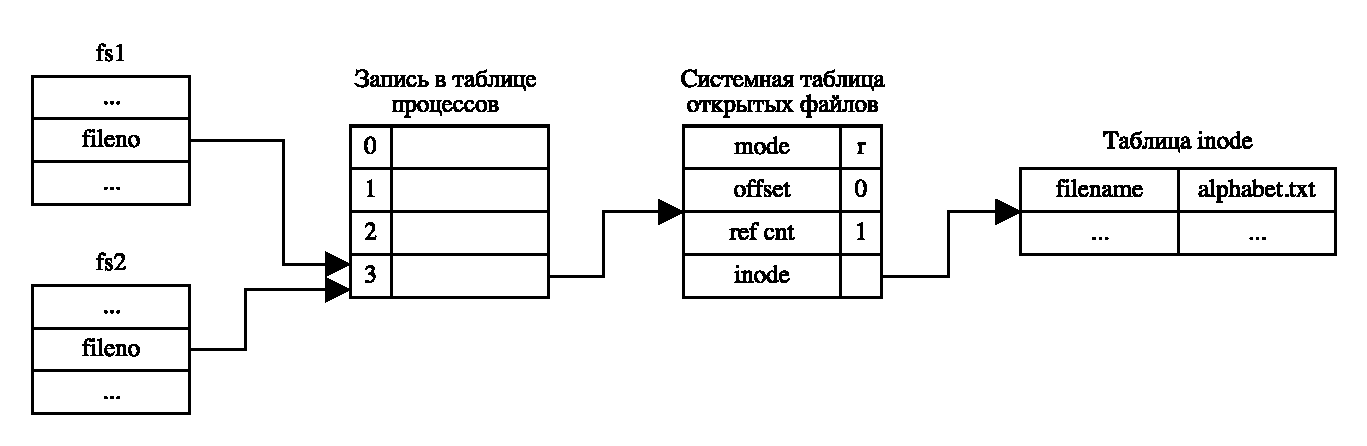
\includegraphics[scale=0.8]{img/1.pdf}
    \caption{Схема связи дескрипторов в программе 1}
\end{figure}

\section{ЗАДАНИЕ 2}

\begin{lstlisting}[caption=Текст программы задания 2]
#include <fcntl.h>
#include <unistd.h>

int main()
{
    char c;
    int cond1 = 1, cond2 = 1;
    int fd1 = open("alphabet.txt", O_RDONLY);
    int fd2 = open("alphabet.txt", O_RDONLY);

    while(cond1 || cond2)
    {
        if ((cond1 = read(fd1, &c, 1)) == 1)
            write(1, &c, 1);

        if ((cond2 = read(fd2, &c, 1)) == 1)
            write(1, &c, 1);
    }

    return 0;
}
\end{lstlisting}

\begin{figure}[H]
    \centering
    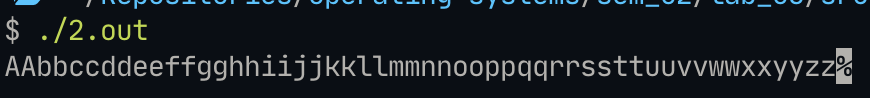
\includegraphics[scale=1.0]{img/2.png}
    \caption{Результат работы программы 2}
\end{figure}

В данной программе создается два файловых дескриптора и, соответственно, две
разные записи в таблице открытых файлов. Поскольку это два разных файловых
дескриптора, то положения указателей в них будут независимы. В результате
получается, что на каждой итерации цикла выводится два одинаковых символа.
Получаем соответствующий результат с дублирующимися символами.

\begin{figure}[H]
    \centering
    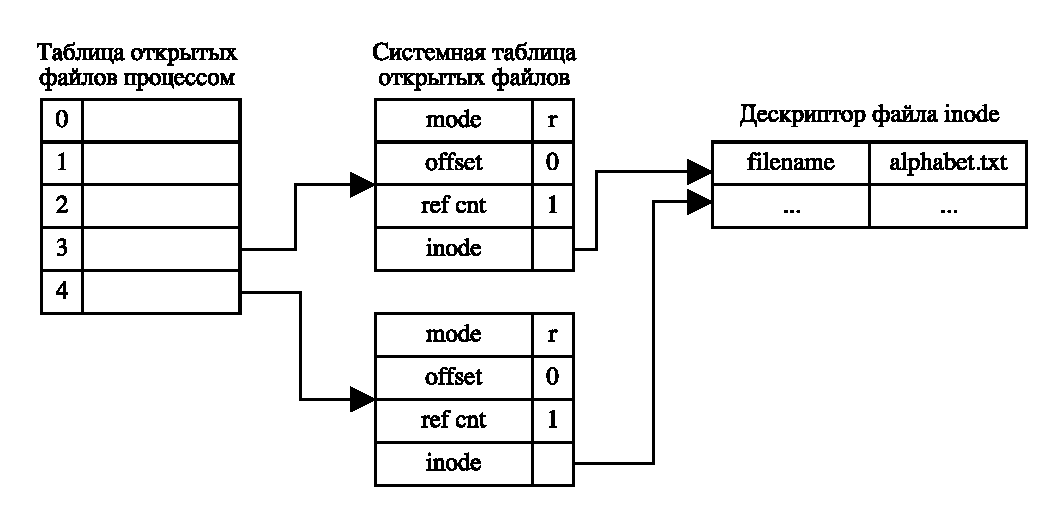
\includegraphics[scale=0.8]{img/2.pdf}
    \caption{Схема связи дескрипторов в программе 2}
\end{figure}

\section{ЗАДАНИЕ 3}

\begin{lstlisting}[caption=Текст программы задания 3]
#include <stdio.h>

int main()
{
    const char letters[] = "Abcdefghijklmnopqrstuvwxyz";
    FILE *fd[2];
    fd[0] = fopen("out.txt", "wr");
    fd[1] = fopen("out.txt", "wr");

    for (int i = 0; i < sizeof(letters) - 1; ++i)
    {
        fprintf(fd[i % 2], "%c", letters[i]);
    }

    fclose(fd[0]);
    fclose(fd[1]);

    return 0;
}
\end{lstlisting}

\begin{figure}[H]
    \centering
    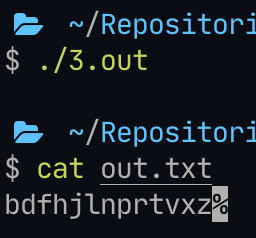
\includegraphics[scale=1.3]{img/3.png}
    \caption{Результат работы программы 3}
\end{figure}

С помощью функции {\ttfamily fopen()} открываются два потока на запись. Два
потока имеют разные файловые дескрипторы, а, следовательно, независимые указатели
в файле. После открытия файлов, в цикле поочередно выводятся символы в разные
потоки. Четные (с индексами 0, 2, 3 и т.д.) записываются в первый буфер,
это буквы a, c, e, g и т.д. Нечетные (с индексами 1, 3, 5 и т.д.) записываются
во второй буфер, это буквы b, d, f и т.д.

Функция {\ttfamily fprintf()} организует буферизованный вывод,
поэтому предполагается, что данные записаны в файл, но реально данные еще
там отсутствуют.

Затем происходит вызов функции {\ttfamily fclose()} для каждого буфера. Эта
фукнция отделяет поток от файла. Если поток использовался для вывода, то
все данные, содержащиеся в буфере принудительно запишутся в файл с использованием
функции {\ttfamily fflush()}.
Поскольку оба потока открыты на запись, то
после выполнения второго {\ttfamily fclose()}, данные, записанные в файл из
первого потока, будут перезаписаны данными из второго. Поэтому в файле
мы увидим буквы b, d, f и т.д.

\begin{figure}[H]
    \centering
    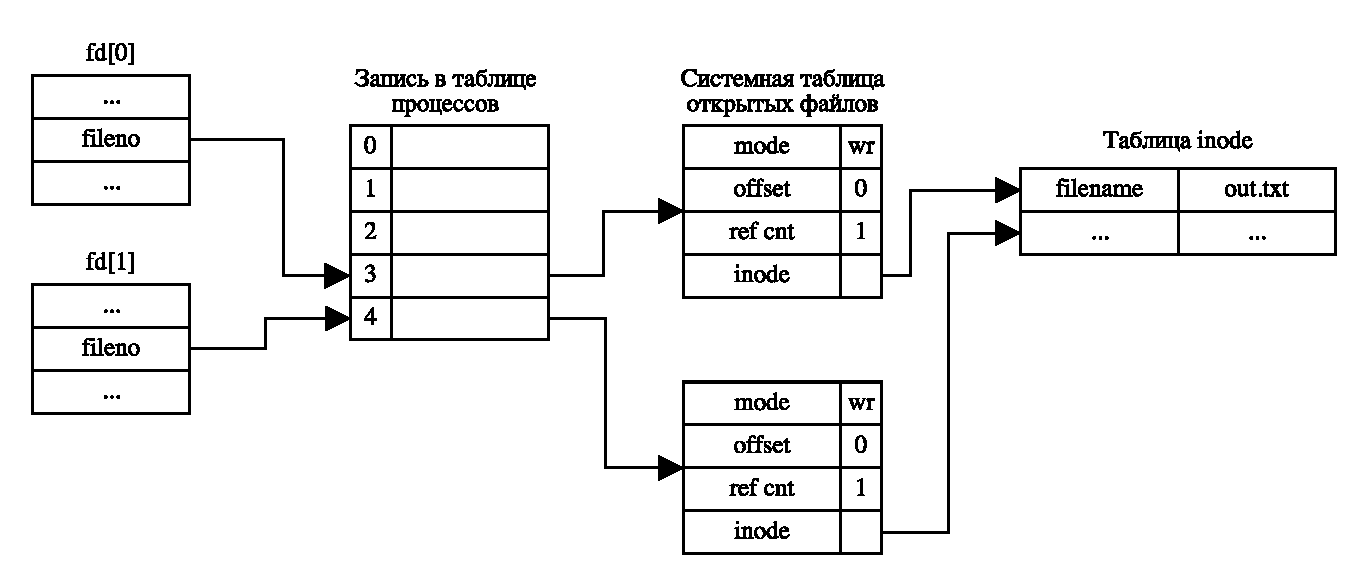
\includegraphics[scale=0.8]{img/3.pdf}
    \caption{Схема связи дескрипторов в программе 3}
\end{figure}

\section{СТРУКТУРА FILE}

\begin{lstlisting}[caption=Структура {\ttfamily \_IO\_FILE}]
struct _IO_FILE
{
  int _flags;       /* High-order word is _IO_MAGIC; rest is flags. */
  /* The following pointers correspond to the C++ streambuf protocol. */
  char *_IO_read_ptr;        /* Current read pointer */
  char *_IO_read_end;        /* End of get area. */
  char *_IO_read_base;        /* Start of putback+get area. */
  char *_IO_write_base;        /* Start of put area. */
  char *_IO_write_ptr;        /* Current put pointer. */
  char *_IO_write_end;        /* End of put area. */
  char *_IO_buf_base;        /* Start of reserve area. */
  char *_IO_buf_end;        /* End of reserve area. */
  /* The following fields are used to support backing up and undo. */
  char *_IO_save_base; /* Pointer to start of non-current get area. */
  char *_IO_backup_base;
  /* Pointer to first valid character of backup area */
  char *_IO_save_end; /* Pointer to end of non-current get area. */
  struct _IO_marker *_markers;
  struct _IO_FILE *_chain;
  int _fileno;
  int _flags2;
  __off_t _old_offset; /* This used to be _offset but it's too small.  */
  /* 1+column number of pbase(); 0 is unknown. */
  unsigned short _cur_column;
  signed char _vtable_offset;
  char _shortbuf[1];
  _IO_lock_t *_lock;
#ifdef _IO_USE_OLD_IO_FILE
};
\end{lstlisting}

\begin{lstlisting}[caption={\ttfamily typedef} в файле {\ttfamily FILE.h}]
typedef struct _IO_FILE FILE;
\end{lstlisting}
